\documentclass[xcolor=dvipsnames]{beamer}
\usepackage{graphicx} 
\usepackage{tabularx}
\usepackage{array}
\usepackage{booktabs} 
\usepackage{listings}
\usepackage{bera}
\usepackage{amsmath}
\usepackage{xcolor}
\usepackage{multicol}
\definecolor{codegreen}{rgb}{0,0.6,0}
\definecolor{codegray}{rgb}{0.5,0.5,0.5}
\definecolor{codepurple}{rgb}{0.58,0,0.82}
\definecolor{backcolour}{rgb}{0.95,0.95,0.92}

\mode<presentation>{
    
\definecolor{MSUgreen}{RGB}{0,100,11} 
\usetheme{Boadilla}
\usecolortheme{spruce}
\setbeamercolor{block title}{bg=MSUgreen!10, fg=MSUgreen!60!black}
\setbeamercolor{navigation symbols dimmed}{fg=MSUgreen!40!white}
\setbeamercolor{navigation symbols}{fg=MSUgreen!40!white}
\setbeamertemplate{itemize item}{\color{MSUgreen}\textbullet}
\setbeamercolor{section in toc}{fg=MSUgreen}
\setbeamercolor{section number projected}{bg=MSUgreen,fg=white}
\setbeamercolor{subsection in toc}{fg=MSUgreen}
\setbeamercolor{subsection number projected}{bg=MSUgreen,fg=white}
}
\lstdefinelanguage{WebAssembly}{
    keywords={func, param, result},
    keywordstyle=\color{blue}\bfseries,
    morecomment=[l]{;},
    morecomment=[s]{/*}{*/},
    morestring=[b]",
    sensitive=true
}
\lstdefinelanguage{HLCostLan}{
    keywords= {service,struct,fn, call, if, else, return},
    keywordstyle = \color{blue}\bfseries,
    sensitive=true,
    morestring=[b]",
}
\lstdefinestyle{custombeamer}{
    backgroundcolor=\color{backcolour},   
    commentstyle=\color{codegreen},
    keywordstyle=\color{blue},
    numberstyle=\tiny\color{codegray},
    stringstyle=\color{codepurple},
    basicstyle=\ttfamily\footnotesize,
    breakatwhitespace=false,
    breaklines=true,
    captionpos=b,
    keepspaces=true,
    numbers=left,
    numbersep=5pt,
    showspaces=false,
    showstringspaces=false,
    showtabs=false,
    tabsize=2
}

\graphicspath{ {../img/} }

\title[CostCompiler]{Un prototipo per lo scheduling di funzioni basato su analisi di costo in piattaforme serverless}
\author{Simone Boldrini}
\date{14 Marzo 2024}
\institute[]{Alma Mater Studiorum - Università di Bologna \\ Facoltà di Scienze}

\begin{document}

\lstset{style=custombeamer}

\begin{frame}
    \titlepage
\end{frame}

\begin{frame}
    \frametitle{Introduzione}
    \alert{Obiettivo}: Sviluppare un compilatore per funzioni serverless che sfrutti tecniche di analisi di costo per ottimizzare l'esecuzione.
    \begin{itemize}
        \item<1-> Definizione di HLCostLan
        \item<2-> Analisi del programma
        \item<3-> Generazione equazioni di costo 
        \item<4-> Generazione del codice WASM
    \end{itemize}
\end{frame}
\begin{frame}
    \frametitle{APP Schema}
    \begin{figure}
        \centering
        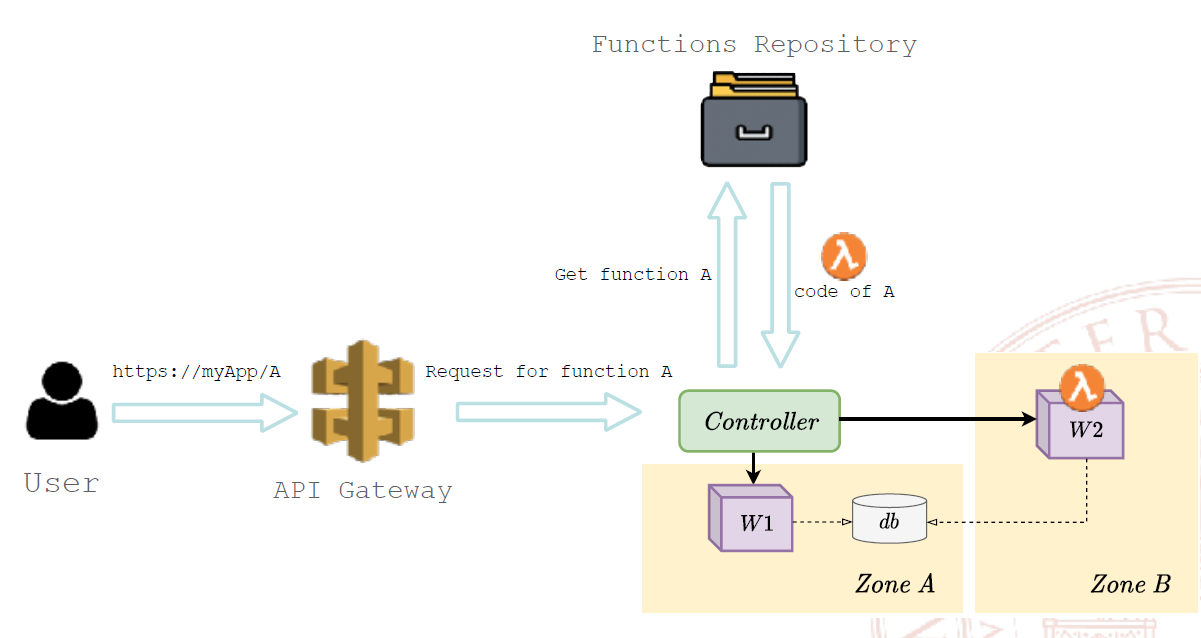
\includegraphics[width=0.9\textwidth]{app_schema.png}
    \end{figure}
    
\end{frame}
\begin{frame}
    \frametitle{Esempio cAPP + CostCompiler}
    \begin{figure}
        \centering
        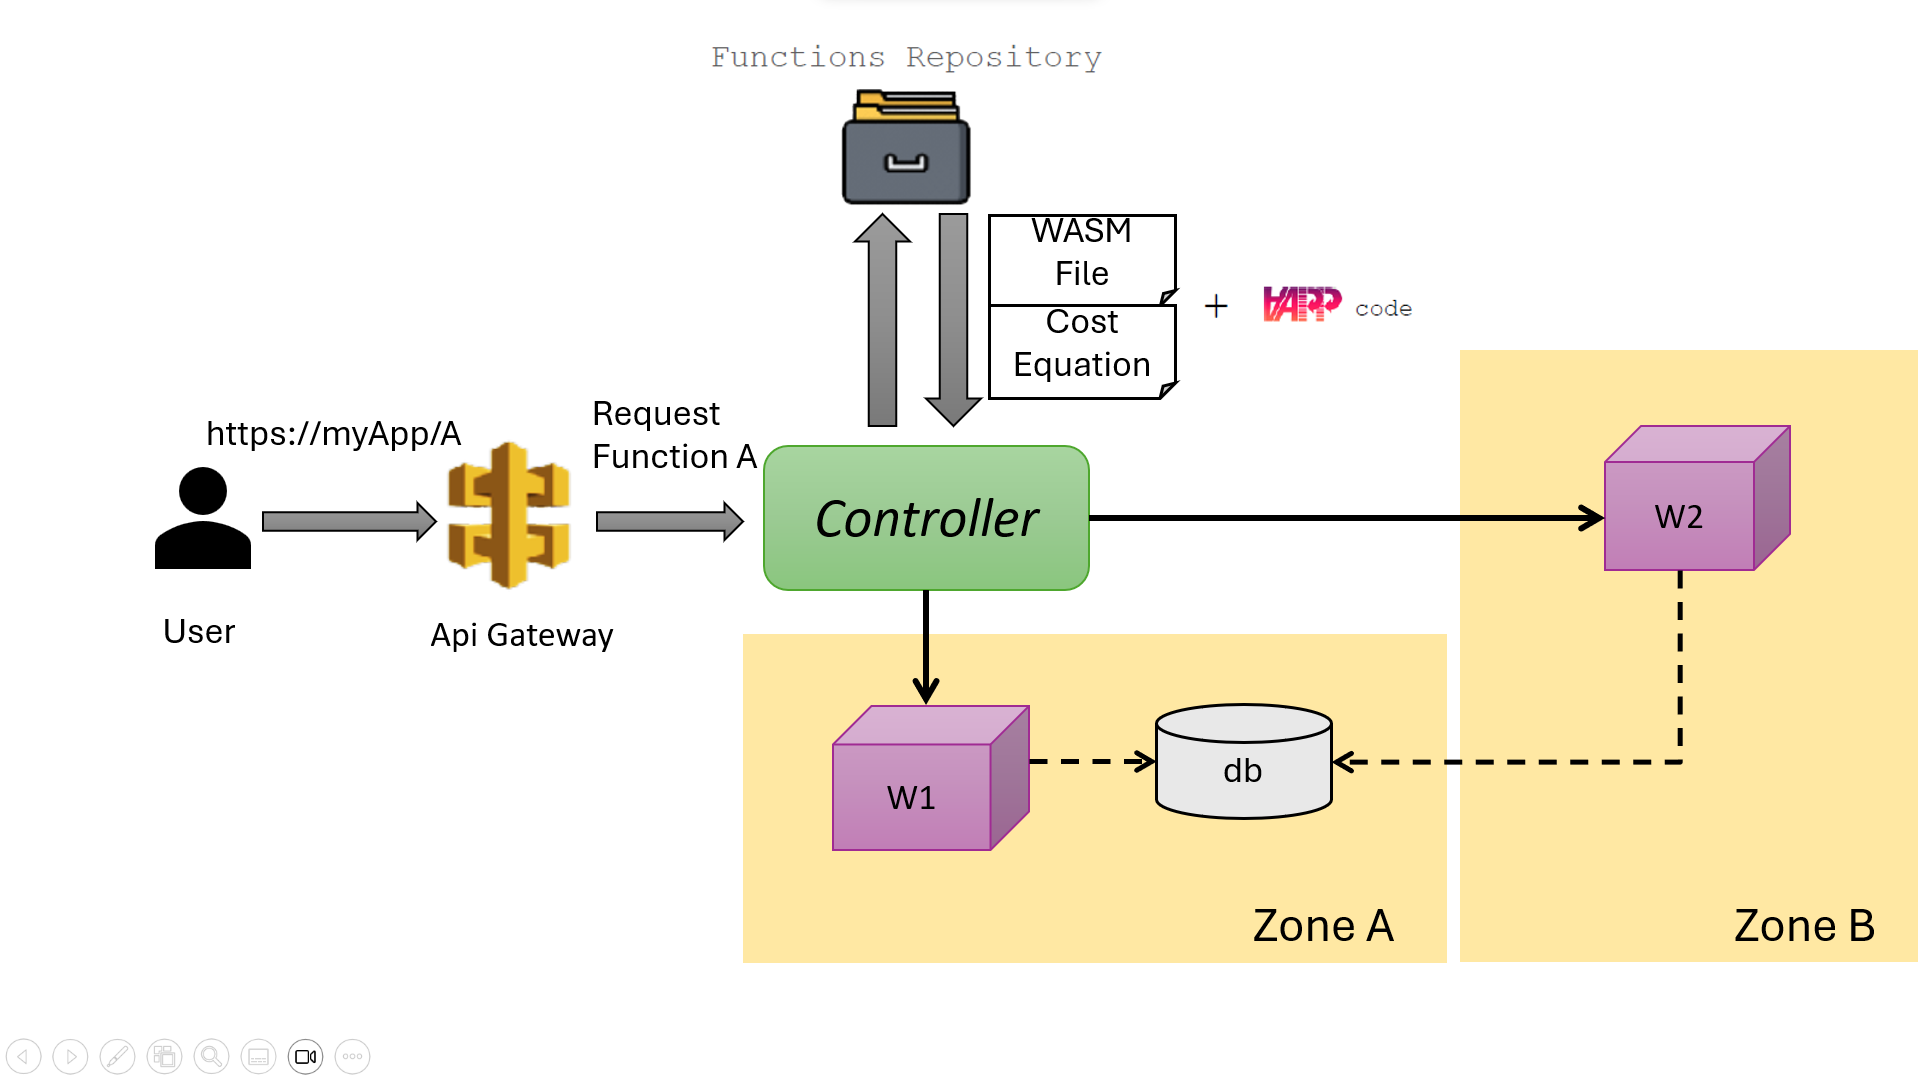
\includegraphics[width=0.9\textwidth]{capp_schema_wasm.png}
    \end{figure}
\end{frame}

\begin{frame}
    \frametitle{Esempio cAPP + CostCompiler}
    \begin{figure}
        \centering
        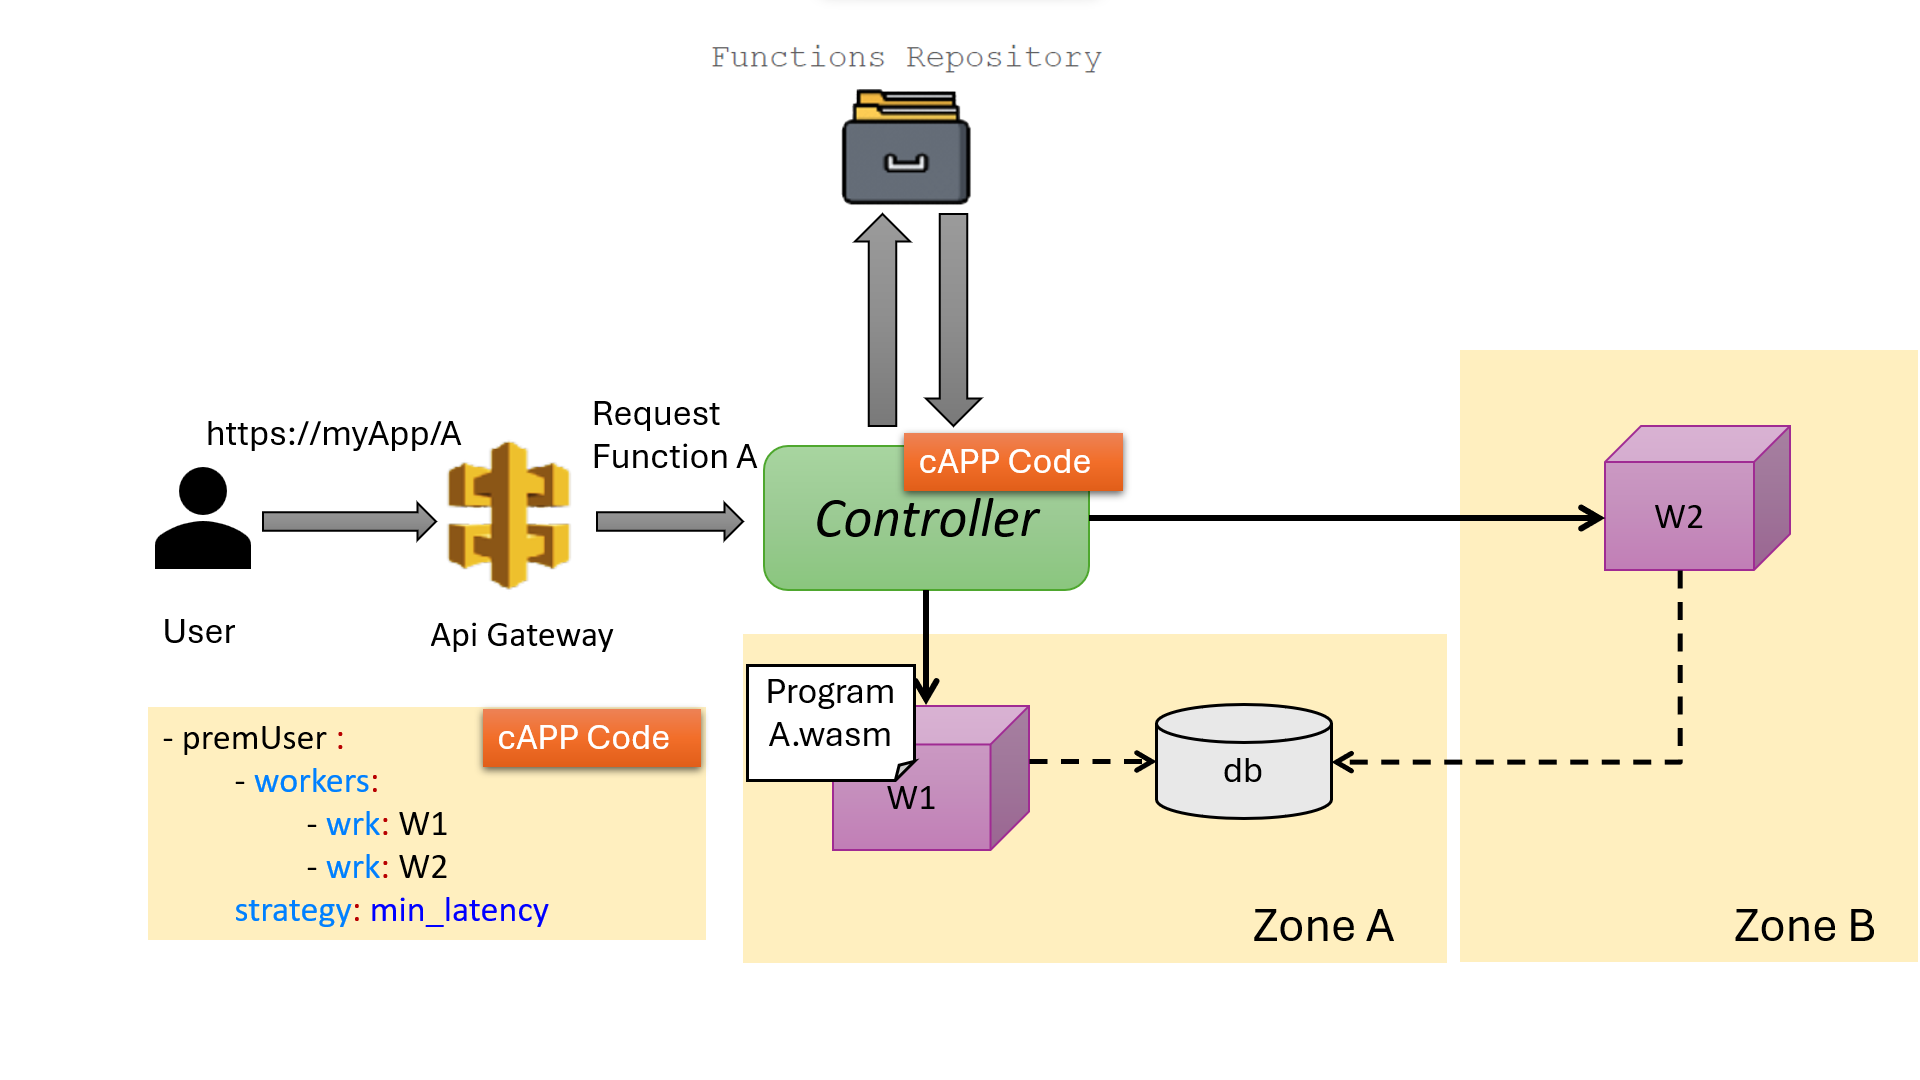
\includegraphics[width=0.9\textwidth]{capp_schema_worker_sel.png}
    \end{figure}
\end{frame}
\begin{frame}
    \frametitle{CostCompiler Schema}
    \begin{figure}
        \centering
        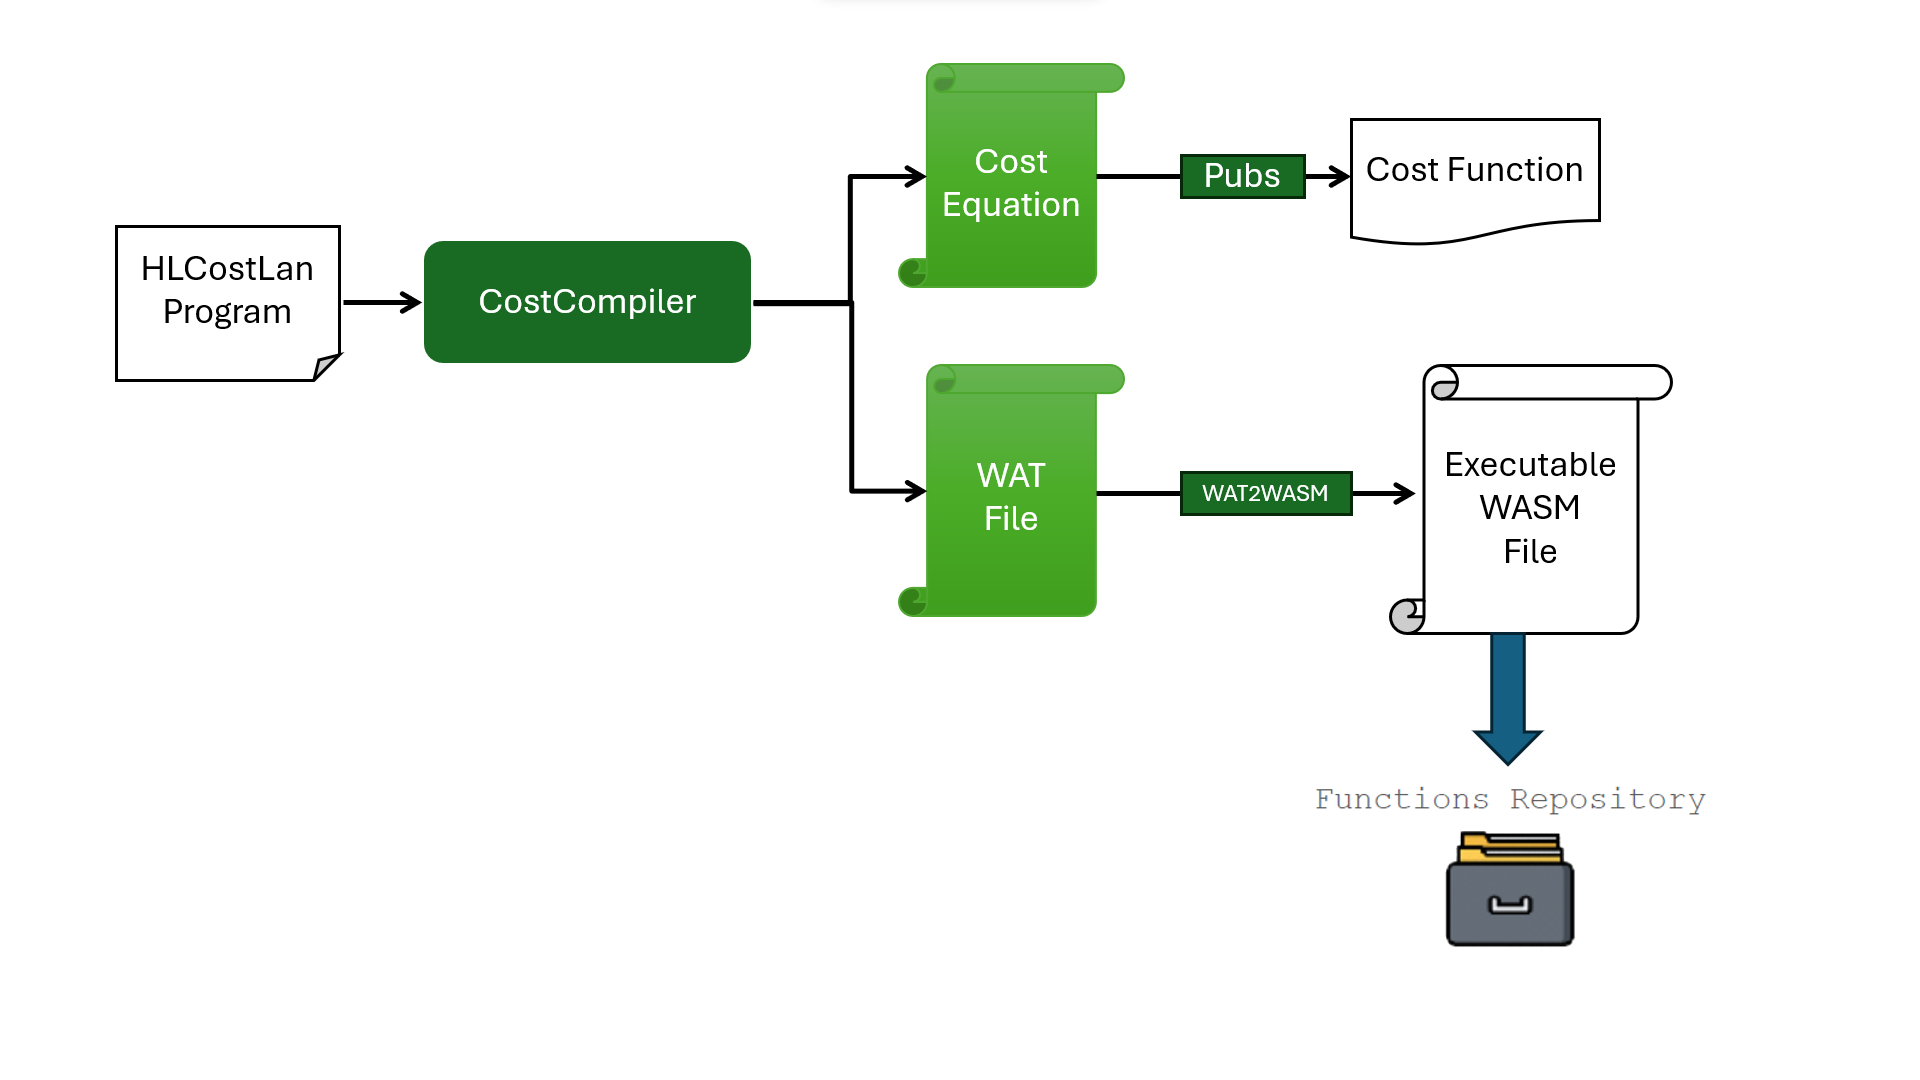
\includegraphics[width=0.9\textwidth]{cost_compiler_schema.png}
    \end{figure}
\end{frame}
\begin{frame}[fragile]
    \frametitle{Esempio di funzioni in HLCostLan}
    \begin{lstlisting}[language=HLCostLan, caption={Listing8}]
    struct Params {
        address: array[int],
        payload: any,
        sender: string
    }
    service PremiumService : (string) -> void;
    service BasicService : (any) -> void;
    (isPremiumUser: bool, par: any) => {
        if ( isPremiumUser ) {
            call PremiumService("test");
        } else {
            call BasicService( par);
        }
    }
    \end{lstlisting}
\end{frame}

\begin{frame}
    \frametitle{Analisi di costo}
    \begin{itemize}
        \item Il compilatore ritorna un insieme di equazioni di costo, che sono adeguate per un Cost-Analyzer.
        \item Il Cost Analyzer scelto è PUBS
        \item I risultati vengono presi dal sistema cAPP permettendo l'allocazione degli scheduling ottimali per le piattaforme serverless.
    \end{itemize}
    
\end{frame}

\begin{frame}
    \frametitle{Analisi di costo}
    Un'analisi di costo è fortemente dipendente dal modello di costo preso in considerazione:
    \begin{itemize}
        \item \alert{Costo di esecuzione}: il costo di esecuzione di una funzione
        \item \alert{Costo di allocazione}: il costo di allocazione di una variabile nell'heap
        \item \alert{Costo di latenza}: il costo di latenza nell'invocazione di una funzione
    \end{itemize}
    I vantaggi delle equazioni di costo:
    \begin{itemize}
        \item Sono \alert{indipendenti} dal linguaggio di programmazione
        \item Possono rappresentare diverse classi di \alert{complessità}
        \item Possono catturare una varietà di nozioni non banali di risorse.
    \end{itemize}
\end{frame}
\begin{frame}[fragile]
    \frametitle{Esempio Cost Equation}
\begin{lstlisting}[language=Java, caption={Equazioni di costo per Listing 8}]
eq(main(P,ISPREMIUMUSER0,B),0,[if9(ISPREMIUMUSER0,P,B)],[]).
eq(if9(ISPREMIUMUSER0,P,B),nat(P),[],[ISPREMIUMUSER0=1]).
eq(if9(ISPREMIUMUSER0,P,B),nat(B),[],[ISPREMIUMUSER0=0]).
\end{lstlisting}
Eseguendo PUBS infine otteniamo:\\
\bigskip
$pubs\_aux\_entry$(A,B,C) -- THE MAIN ENTRY

  * Non Asymptotic Upper Bound: max([nat(C),nat(A)]) 
\end{frame}
\begin{frame}
    \frametitle{Generazione del codice WASM}
    Una volta ottenute le equazioni di costo, abbiamo sviluppato un interprete per la generazione del codice WASM.\\

\end{frame}
\begin{frame}
    \frametitle{WebAssembly}
    \alert{WebAssembly} rappresenta una tecnologia versatile e potente che offre un'alternativa efficace alle tradizionali soluzioni di esecuzione di codice.\\
    Le istruzioni \alert{Wasm} si distinguono dalle istruzioni di un processore reale in quanto sono progettate per l'esecuzione in un ambiente virtuale.

\end{frame}
\begin{frame}[fragile]
    \frametitle{Esempio HLCostLan}
    \begin{lstlisting}[language=HLCostLan, caption={Esempio di funzione HLCostLan, Listing15}]
    fn svc(i: int, n:int) -> any{
            return n * i
     }
     (len : int) => {
         return svc(len,4)
     }
    \end{lstlisting}
\end{frame}
\begin{frame}[fragile]
    \frametitle{Equivalente WAT}
    \thispagestyle{empty}
        \begin{lstlisting}[language=WebAssembly]
    (func $svc (param $i i32) (param $n i32) (result i32)
    (local $res i32)
    (if(i32.eq
    (local.get $i)
    (local.get $n))
    (then
    (i32.const 1)
    (local.set $res))
    (else
    (i32.const 0)
    (local.set $res))
    )(local.get $res))

    (func $main (export "main")(param $a i32)(param $b i32) (result i32)
    (local.get $a)
    (local.get $b)
    (call $svc)
    )
        \end{lstlisting}
\end{frame}
%\begin{frame}
%    \frametitle{Vantaggi e Svantaggi di WASM}
%    \begin{multicols}{2}
%         \alert{Vantaggi}:
%        \begin{itemize}
%            \item \alert{Velocità}: progettato per essere eseguito in modo efficiente su hardware moderno.
%            \item \alert{Sicurezza}: progettato per essere eseguito in un ambiente sandbox.
%            \item \alert{Portabilità}: progettato per essere eseguito su qualsiasi piattaforma.
%        \end{itemize}
%        \columnbreak
%        \alert{Svantaggi}:
%        \begin{itemize}
%            \item \alert{Complessità}:linguaggio a basso livello, quindi è più difficile da scrivere e leggere rispetto ad altri linguaggi.
%            \item \alert{Mancanza di supporto}:  è relativamente nuovo, quindi non tutti i browser e le piattaforme lo supportano.
%        \end{itemize}
%          \end{multicols}
%\end{frame}
\begin{frame}
    \frametitle{Conclusioni}
    \begin{itemize}
        \item É stato sviluppato un \alert{interprete prototipale} attraverso il quale è possibile eseguire programmi scritti in HLCostLan.
        \item L'interprete offre la possibilità di derivare \alert{l'equazione di costo} associata a tali programmi
        \item CostCompiler genera automaticamente il corrispondente codice \alert{WebAssembly}.
    \end{itemize}
\end{frame}

\begin{frame}
    \frametitle{Sviluppi Futuri}
    \begin{itemize}
        \item Integrazione con Kubernetes
        \item Estendere il linguaggio HLCostLan
        \item Condurre studi sperimentali e valutazioni empiriche per testare l'efficacia del sistema in scenari realistici di utilizzo
    \end{itemize}
    

\end{frame}
\end{document}